%!TEX root = ../Thesis.tex
\chapter{UAV prototype - system description}
This chapter describes the working principle, the physical prototype of the drone, its electrical electronics parts.

\section{Overview}
 
The prototype is a coaxial contra-rotating copter drone. For thrust, it features two propellers placed on z axis of the drone (longitudinal), rotating in the opposite direction to each other. 
This concept was adopted because a single propeller would introduce a moment in the frame about its axis in the opposite direction of its rotation, while having two contra rotating propellers cancel each other’s axial introduced moments. 
 The advantages of using such a machine are its reduced scale, thrust-to-weight ratio,  and  aerodynamic symmetry, which removes the yaw moment and side forces commonly seen in single-rotor copters. \cite{wang2014flight} 
 The main components of the drone are the metal frame, the two propellers, a metal rudder, the Arduino and IMU.
 

 \section{Drone building and assembly process}

The building of the drone required considerable machining and production work. 
It was decided on aluminium rectangular plates and four aluminium legs for the drone in order to be statically stable. The material was chosen in order to be light. 
The frame plates were measured and designed in CAD drawing (Figures \ref{fig:CAD}, \ref{fig:CADfront}, \ref{fig:CADback}). A CNC plasma cutter custom built in the workshop cut the frame out of aluminium plates. 

\begin{figure}[h]
  \centering
  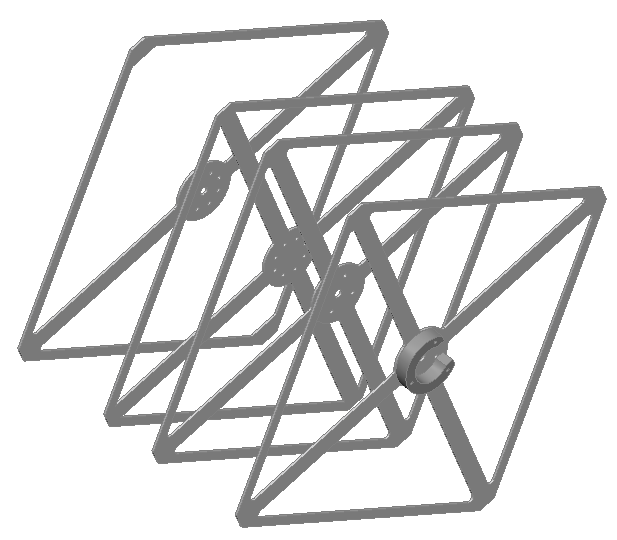
\includegraphics[scale=0.6]{graphics/droneCAD2.png}
  \caption{UAV frame CAD}
  \label{fig:CAD}
\end{figure}


\begin{figure}[h!]
  \centering
  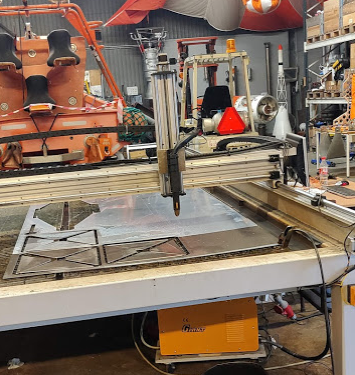
\includegraphics[scale=0.9]{graphics/CNCmachine.png}
  \caption{CNC plasma cutting of the aluminium frame}
  \label{fig:CNC plasma cutting}
\end{figure}


The plasma cut aluminium plates had holes drilled, countersunk to allow the motor screws to sit flush. For stability, they were fastened with rivets to aluminium angle profiles, which constituted the legs and the supports for the plates.

\begin{figure}[h!]
  \centering
  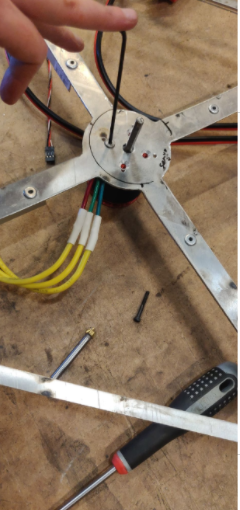
\includegraphics[scale=0.7]{graphics/Drone/Drone.png}
  \caption{Drone assembly}
  \label{fig:Drone assembly}
\end{figure}



For the mounting of propellers and their motors on the plates, two green 3D printed holders that were measured to fit the motors diameter and the opening required to mount the propeller servo motor.

\begin{figure}[h!]
    \centering
    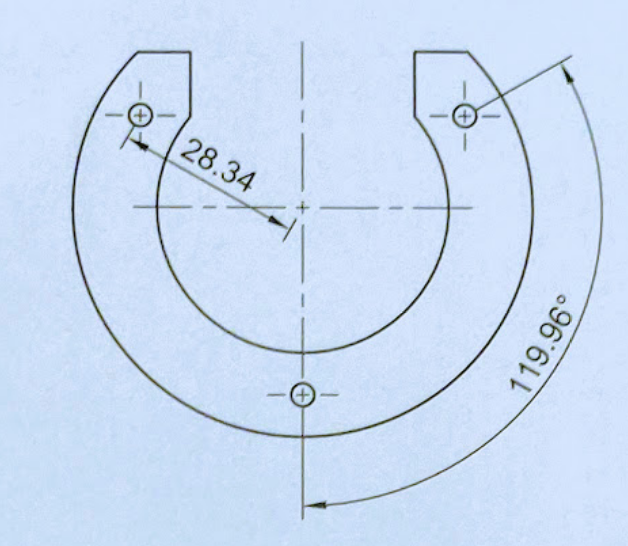
\includegraphics[scale=0.4]{graphics/Drone/ServoHolder.png}
    \caption{3D printed motor holders drawing}
     \label{fig:3D printed motor holders drawing}
\end{figure} 

The holders were drilled manually to avoid breaking the material and mounted such that it allowed for the correct installation and movement of the propellers, that is, allowed their servo motor (pictured) to adjust the pitch of the propellers. 
Once the servo was mounted, the motors and propellers were mounted with screws on the two top levels of the aluminium frame. 


\begin{figure}[h!]
    \centering
    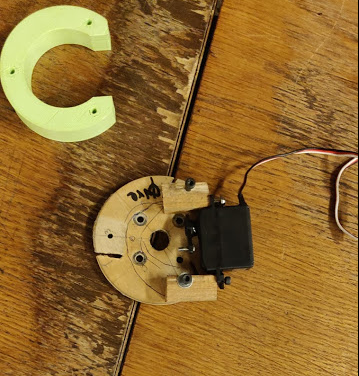
\includegraphics[scale=0.8]{graphics/Drone/GreenHolders.png}
    \caption{3D printed motor holders and propeller servo motor}
     \label{fig:3D printed motor holders and propeller servo motor}
\end{figure} 

 
\section{Electrical components}

The setup has electric supply from a 12V LiPo battery, powering the propeller motors and its transmitters. There is an RC controller commanding the propellers’ motors through the transmitters, with cables connecting the motors to the battery. 
The Arduinos, servo and the IMU are powered by a power source capable of outputting 5 V to the breadboard. This is due to the Arduinos providing insufficient power for running all these components. 

\section{Servo motor}

A servo motor is used to move the rudder, actuating the control system through a middle plastic link connecting the servo arm to the rudder arm.
Some behaviors have been observed in lower cost servos, which negatively affected the system performance and introduced delays or challenges for the controller. 
An important consideration was reducing the servo play observed in some models (backlash), that is, the servo arm not being fastened to its position by its gearbox, but allowing for a sway movement of some degrees and resulting in a deviation at the end of the servo arm. 

This was problematic considering that the rudder is a heavier object that can exert a force strong enough to affect the servo’s arm position, with potential of overpowering a weaker gearbox and taking advantage of this play,  thus impacting the servo’s true position due to its mass during actuation.
This effect would introduce delays and disrupt the performance of the control system by producing an output some degrees away from the commanded one, under the force of the rudder pulling and pushing on the servo arm. 
 
Another observed behaviour in these servos was imprecise position control from the servo’s gearbox controller, which made it noticeable that after sending a position command from Arduino, for example 90 degrees, the servo would overshoot, reaching some degrees over 90, then correcting itself to 90. 
This would pose a problem for the controller, as the angular position it would command would not be the one produced by the servo at the specified time, but rather first overshooting then  correcting itself, adding instability and delay to the system which the controller would have to compensate for. The effect of this overshoot on the drone's pitch angle would be magnified under the force of propellers, causing unnecessary oscillations. 
 
These behaviors were observed in different servos that have been installed and tried for the purpose, with some failing (burning out) after repetitive movement. The final choice was a Futaba servo, which did not exhibit the previously mentioned challenges and which proved to be durable, reliable, more precise and has a demonstrated history for sound aerial performance from previous rocket flights, used for actuating the exhaust vanes against the engine thrust. 
 
\begin{figure}[h!]
    \centering
    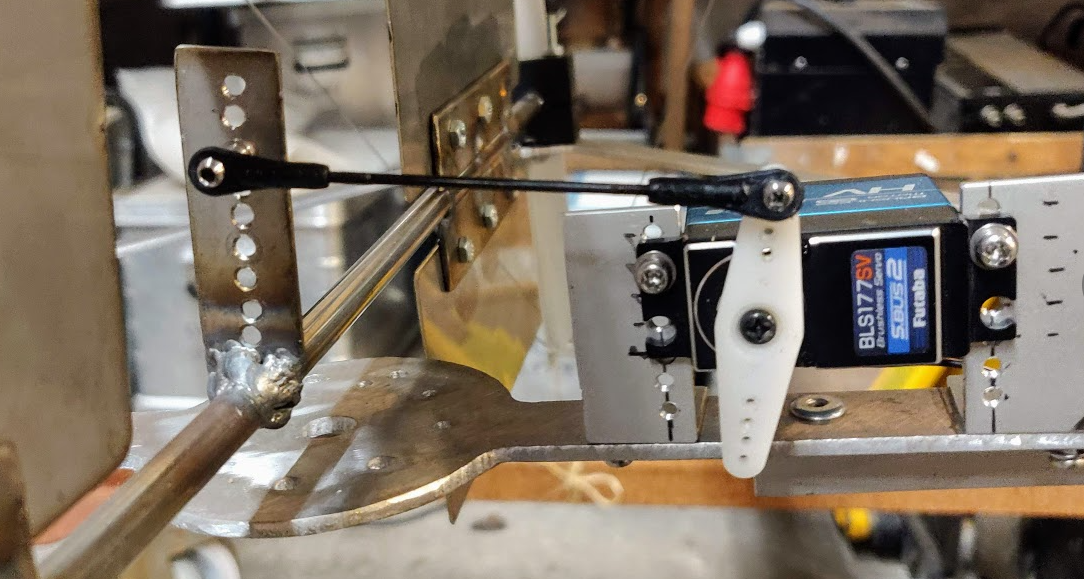
\includegraphics[scale=0.5]{graphics/Drone/Servo.png}
    \caption{Mounted servo motor}
     \label{fig:Mounted servo motor}
\end{figure}  

 
The mounting of the servo involved prior trial and error in order to find the position situated at the midrange of the servo. This was necessary in order to ensure roughly equal movement back and forth. 
In order to find the servo midrange, its position was commanded to 0 degrees, assumed to be the minimum, and to 180, assumed to be the maximum. 
Initially, the servo was tested at 0 degrees, however, some servos were not responding (moving) to set position to 0 degrees, while responding by moving to 90 degrees or higher values. 
 
It was found that while some servos have their starting point from 0 degrees, it was not a general rule.  The Futaba one did not respond to commands of setting position to 0 degrees, as it was discovered to have working range from 30-160 deg. Due to  having a range of motion of 130 degrees, its midpoint was found at 30+130/2=95 degrees. 
The servo was set to its midpoint as initial condition (starting position), then mounted on the frame for future tests. 
 
\section{Rudder}

The rudder serves the purpose of providing thrust vector control by deflecting the flow from the propellers by an angle. 
It was decided to provide control in one degree of freedom only (pitch angle) as a technology demonstrator. 

\begin{figure}[h!]
  \centering
  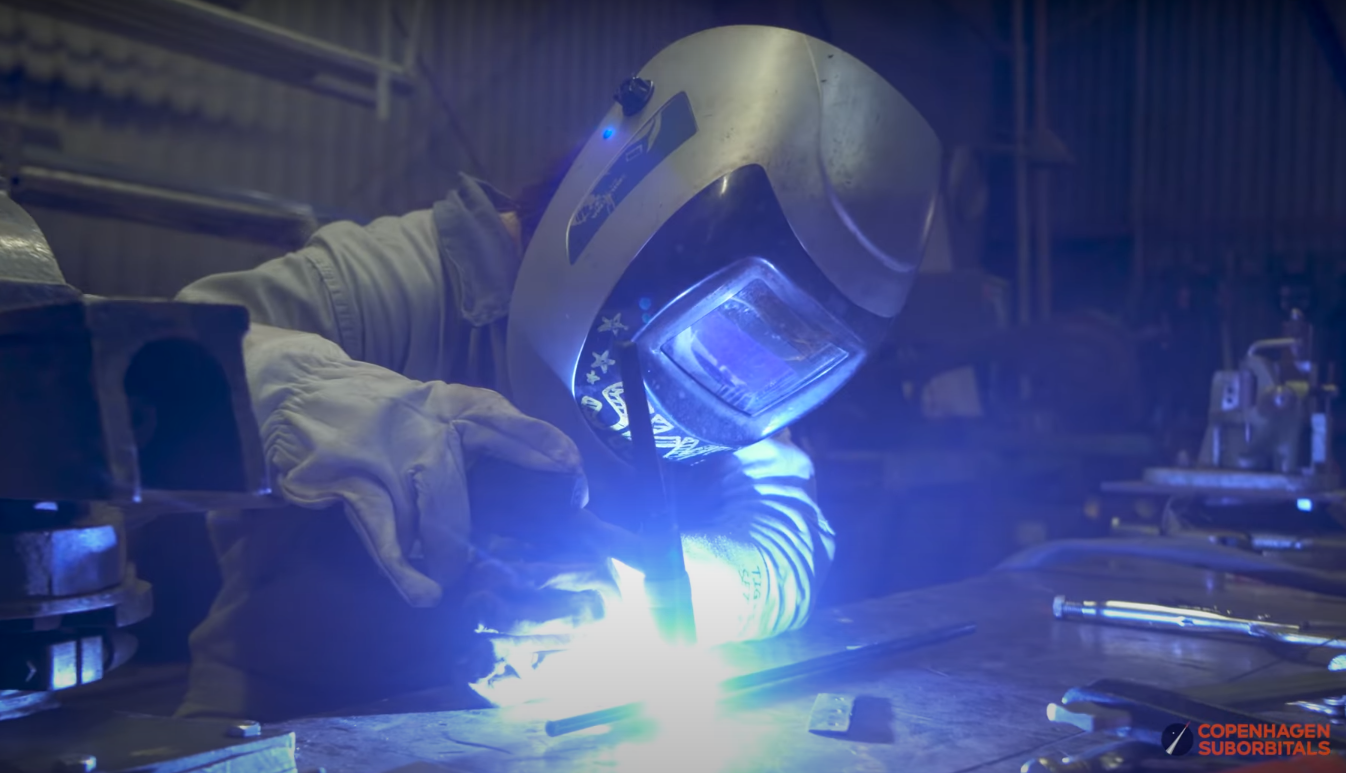
\includegraphics[scale=0.4]{graphics/rudderweld.png}
  \caption{Welding of rudder}
  \label{fig:Rudder TIG welding}
\end{figure}

A steel rod was cut to fit the drone profile and serve as mount and axis for the rudder fins. After measuring for the proper placement of the fins, four rectangular steel pieces were cut, holes machined and TIG welded on the steel rod to support the fins. TIG welding was preferred rather than MIG due to the small size of the pieces and the intent on joining them together through melting as opposed to adding extra material, to keep the mass of the rudder reduced. 

\begin{figure}[H]
  \centering
  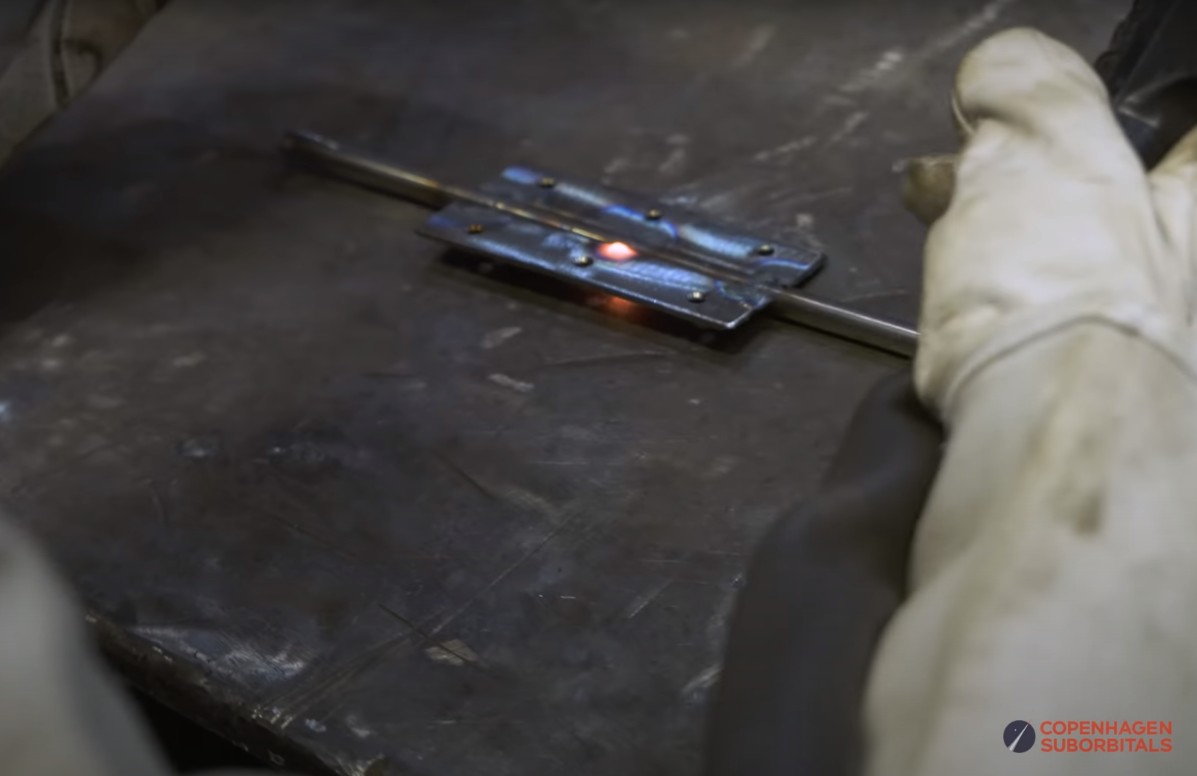
\includegraphics[scale=0.3]{graphics/Drone/weld2.png}
  \caption{TIG welding of rudder}
  \label{fig:TIG welding of rudder}
\end{figure}


There was a need for the rudder to have a connection to the servo motor. For this purpose, another thin piece of metal is attached to the rod perpendicularly to act as an arm. 
The metal piece was designed, cut and had holes drilled 5 mm apart in order to allow for multiple placements for the servo link. The piece was then MIG welded on to the rudder. 

\begin{figure}[h!]
    \centering
    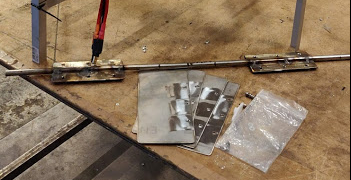
\includegraphics[scale=1.1]{graphics/Drone/RudderPieces.png}
    \caption{Rudder mount and fins}
     \label{fig:Rudder mount and fins}
\end{figure} 


The rod was now assembled ready to be placed on the frame. 
For its placement, two sets of black 3D printed brackets were designed. The brackets were designed to allow the rudder to be mounted and removed easily, by having a detachable top bracket. 
After being produced, and drilled through, the bottom bracket was attached to the bottom aluminium plate and the top one fastens with screws on top.  
The rod with the supporting pieces was then mounted in the two 3D printed brackets, allowing it to move freely along its axis. 
 
The rudder fins were the last pieces to be added to the setup. The fins were produced by having four metal plates were cut, surface polished for easier welding, then drilled, countersunk and mounted with screws on the welded supports - subsequent to installing the rod in the frame. 
Thus, the rudder was completely assembled. The rudder is linked to the servo arm through a thin rigid link, detailed in the modelling section. 

\begin{figure}[h!]
    \centering
    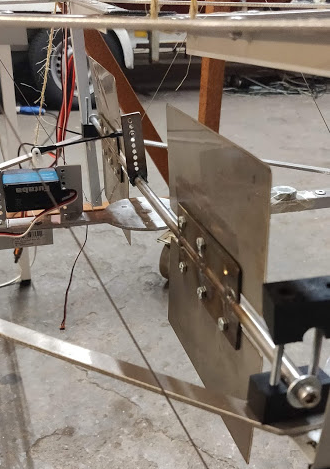
\includegraphics[scale=0.8]{graphics/Drone/rudder.png}
    \caption{Rudder - servo motor assembly}
     \label{fig:Rudder - servo motor assembly}
\end{figure} 

 
 \section{Electronics IMU, Arduino}
 
The IMU is mounted on the plate above the rudder, because that is where the center of mass is located on the drone. 
It sits on a breadboard, attached with Velcro adhesive which serves a double purpose: to mount the IMU in a way that allows for taking it off the drone for testing and calibration, and to dampen vibrations from the propellers when they are running.
The IMU is connected to the Arduino, sitting on the table two meters away, through an extended cable. 
The Arduinos, IMU and servo are connected to a breadboard, powered by the power supply. 

\begin{figure}[h]
  \centering
  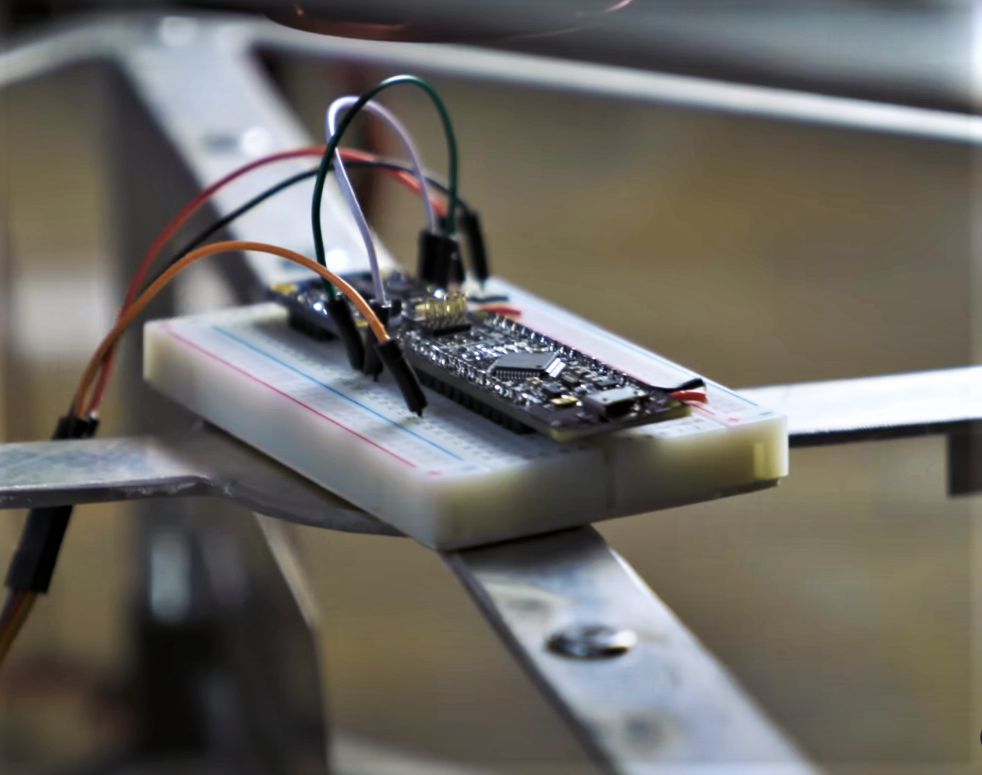
\includegraphics[scale=0.3]{graphics/Drone/ArduinoNano2.png}
  \caption{Arduino Nano}
  \label{fig:Arduino Nano}
\end{figure}


The extension cable was necessary in order to connect the IMU to the microcontroller on the table. 
The cable was made by removing isolation off cable ends, soldering rigid metal piece to the ends in order to ensure it stays fixed on the breadboard; then plastic separator was added to help isolate, with heat gun.
The setup was tested by reading the data coming out of the IMU, to ensure continuity and correct transmission. 
This chapter described the constituent parts of the drone to provide an overview of the “plant” to be controlled, along with introducing the electronics and IMU sensor. Next chapter explains the IMU sensor more in depth in connection with the Arduinos for the purpose of state estimation. 


\begin{figure}[h]
  \centering
  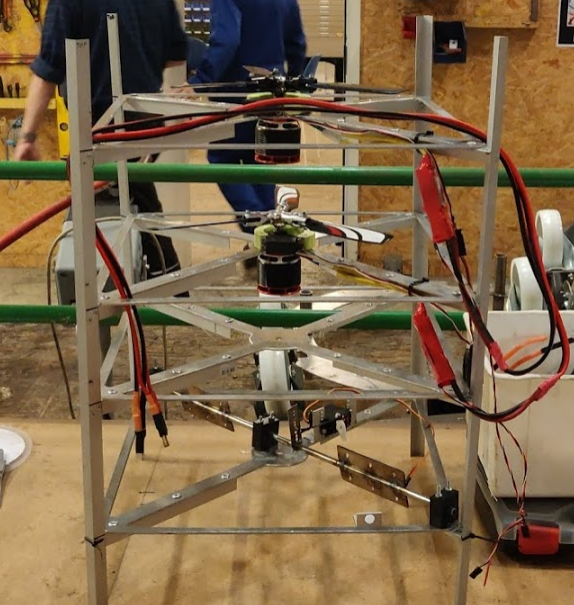
\includegraphics[scale=0.7]{graphics/Drone/droneBuilt.png}
  \caption{Assembled drone}
  \label{fig:Assembled drone}
\end{figure}